
\loadgeometry{include}
\addtocounter{page}{-1}
\thispagestyle{empty}
\begin{center}

\includegraphics[width=\textwidth]{miscpages/title.pdf}
\end{center}
\newpage
\thispagestyle{front}


\loadgeometry{normalinverse}
% \addtocounter{page}{-1}
\ifthenelse {\equal{\ISDEF}{0}}
{} {
\thispagestyle{front}
%\addtocounter{page}{1}



% ------------------------------% ------------------------------%
\chapter*{Avant propos}
%\addcontentsline{toc}{chapter}{Avant propos}
\markboth{Avant propos}{Avant propos}
% ------------------------------% ------------------------------%
L’Université Nazi BONI a été créée le 23 mai 1997. Elle est située à quinze
(15) kilomètres à l’Ouest de Bobo et est composée de six (06) établissements à savoir :
\begin{itemize}
  \item L'Ecole Supérieure d'Informatique(ESI)
  \item L'Institut de Développement Rural(IDR)
  \item l'Institut Nationale des Sciences de la Santé(INSSA)
  \item l'Institut Universitaire de Technologie(IUT)
  \item l'UFR Sciences Juridique Politique Economique et Gestion(UFR SJPEG)
  \item l'UFR Sciences et Technologies(UFR ST)
  \item l'UFR Sciences Humaines, Lettres, Arts, et Communication(UFR SH-LAM)
\end{itemize}

L'ESI a pour mission d'accompagner le Burkina Faso dans sa transformation
digitale. Pour cela, elle forme depuis sa création des cadres supérieurs en
informatique qui font sa fierté dans toutes le administrations du pays.

Afin de préparer les futurs diplômés à l’insertion dans la vie professionnelle,
l'ESI prévoit que chaque futur diplômé effectue un stage de fin de cycle
dans une entreprise ou dans un centre de recherche ou de développement.

C’est dans ce contexte, que nous avons été reçu au LIRIS pour notre stage de fin de cycle.
Le présent document fait office de memeoire des travaux que nous y avons menés.

\thispagestyle{front}
%\addtocounter{page}{2}
%%  une page de citation (pas indispensable)
 \vspace{\stretch{1}}
\vspace{0.5\linewidth}
\begin{flushright}
  %\emph{No physical quantity can continue to change exponentially forever. Your job is delaying forever.}\\
  \emph{}\\
  
\end{flushright}
\vspace{\stretch{2}}

%% Encore une page blanche pour que les remerciements arrivent
%%  sur une page impaire

\thispagestyle{front}
%\addtocounter{page}{3}
\chapter*{Dédicace}

\vspace*{\stretch{1}}
\begin{flushright}
  A  \\
  Mes parents\\
  \textbf{Monsieur \textsc{DABONNE} Hanido}\\ Et  \\
  \textbf{Madame \textsc{DABONNE} Née BALIMA Habibou}\\
  \normalsize Je ne vous remercirais jamain assez pour tout ce que vous avez fais 
  pour moi au quotidient. Soyez en remercier\\
  \textbf{Madame \textsc{DABONNE} née \textsc{COMOE} Maouwa}\\
  \normalsize Que ton ame repose en paix. 


  A ma bousole  \\
  \textbf{Monsieur \textsc{DABONNE} Ousseni}\\
  \normalsize Ton acharmement et ta determination au travail font de toi ma source
   d'inspiration et mon modèle. Merci de toujours me montrer le chemain de la droiture.
\end{flushright}

\vspace*{\stretch{2}}

\thispagestyle{front}
%\addtocounter{page}{4}

%\remerciements
\chapter*{Remerciements}

La redaction de ce memoire a été possible grace a plusieures personne et institution à qui je voudrais 
temoigner ma gratitude et mes sincères reconnaissances:

  Je tiens à remercier le programme Erasmus+
  pour m'avoir donner cette chance de sejourner en France et de faire mon stage 
  dans l'un des plus grands laboratioire francais. 
  
  
  Je remercier \textbf{Professeur Serge \textsc{Miguet}} et \textbf{Professeur Mihaela \textsc{Scuturici}}
    mes tuteur de stage, pour les conseils et suggestions, combien précieux dans la
    réalisation de notre travail;
  
  Je desire remercier \textbf{Professeur Tigiane\textsc{Yelemou}} mon tuteur accademique
  pour ces conseils et suggestions.
 
  Un grand merci à \textbf{Professeur Pasteur \textsc{Poda}}, coordonateur de notre master
    pour son don de soit dans le bon deroulement de notre formation.

  En fin, je tien à remercier l'ensemble du corps professoral et administratif de l'ESI  pour toute la
    disponibilité et l'encadrement dont nous avons bénéficié.
  
A tous ceux qui ont contribué d'une manière ou d'une autre à la réalisation de
ce travail, MERCI.

\thispagestyle{front}
%\addtocounter{page}{5}
}

\begin{center}
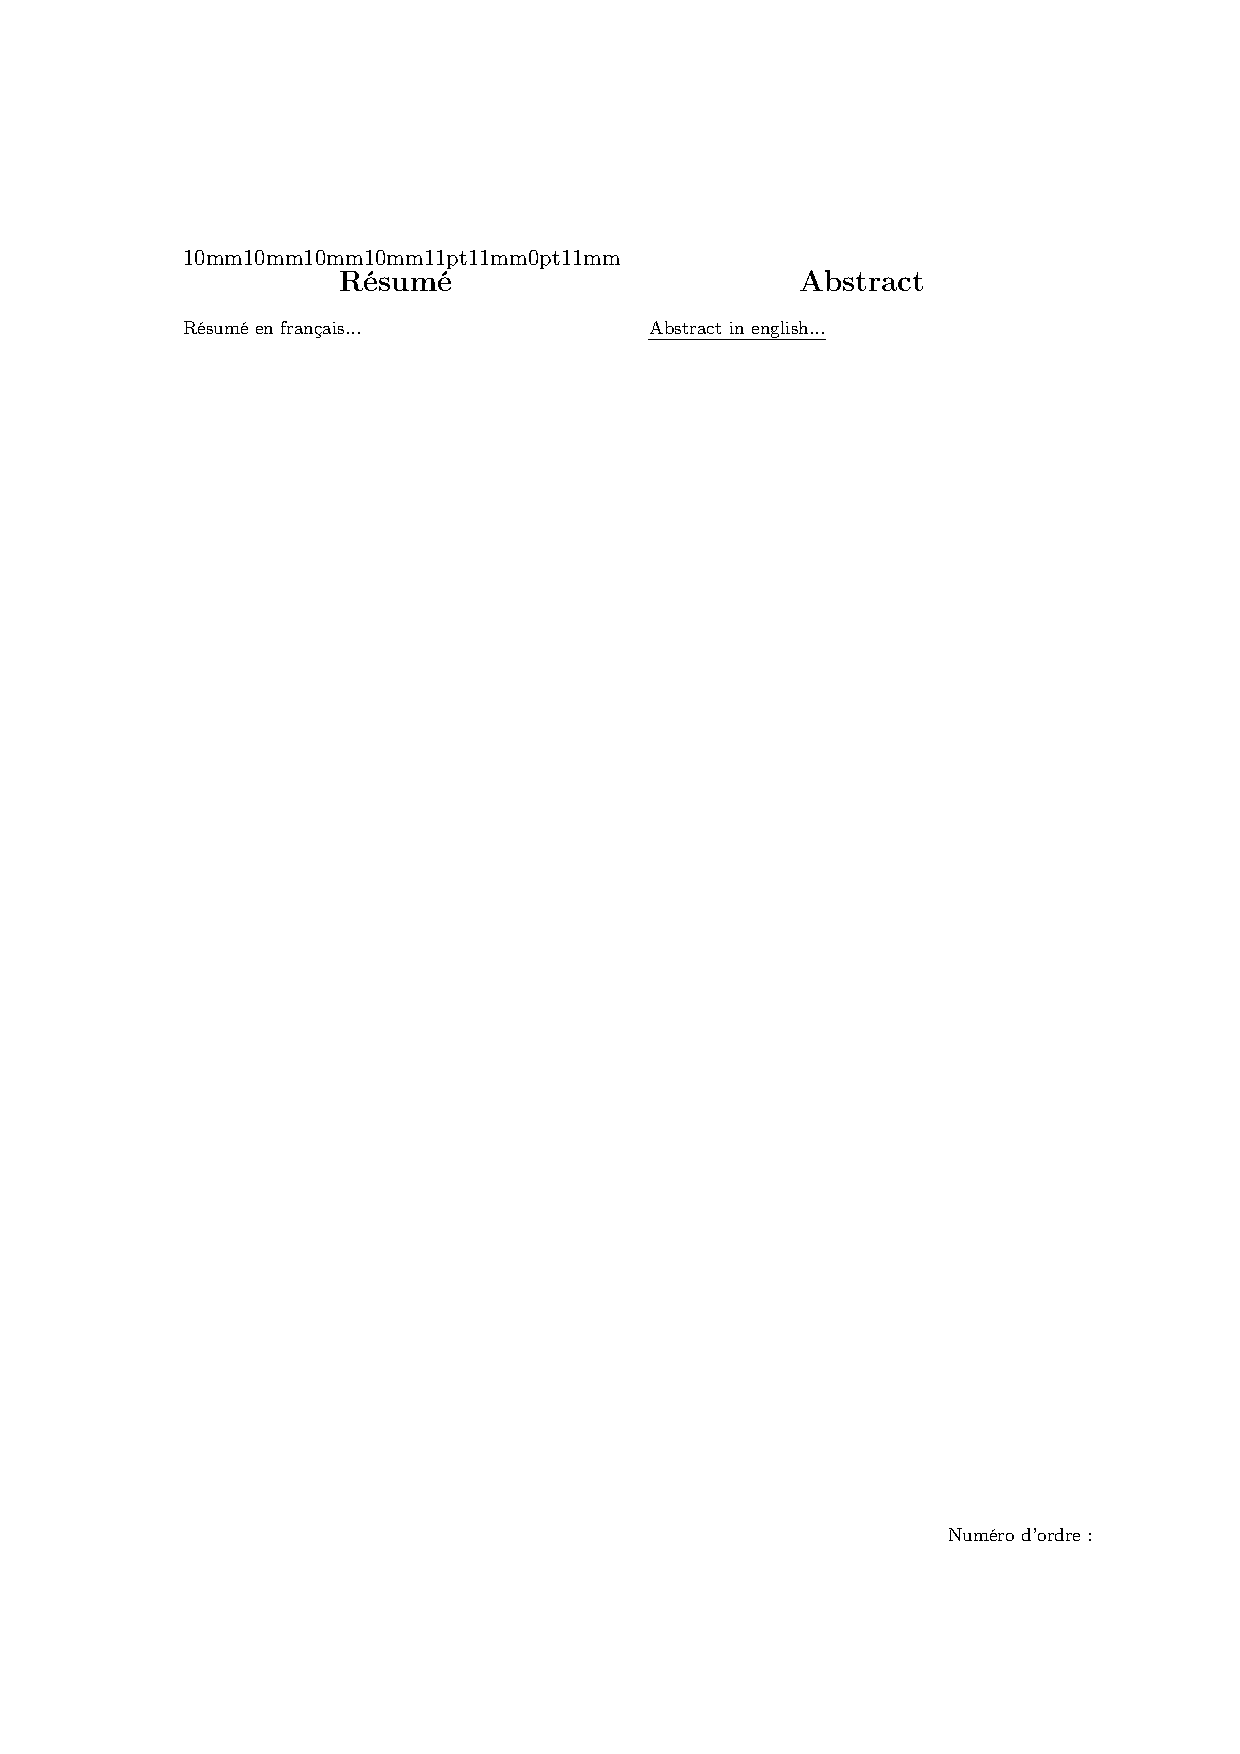
\includegraphics[width=\textwidth]{miscpages/resume.pdf}
\end{center}


